\documentclass[a4paper,ngerman,12pt]{exam}
\usepackage{babel}
\usepackage[utf8]{inputenc}
\usepackage[T1]{fontenc}
\usepackage{graphicx}
\usepackage{algpseudocode}
\usepackage{geometry}
\usepackage{csquotes} % Anführungszeichen
\usepackage{paralist} % kompakte Aufzählungen
\usepackage{textcomp,tikz} %diverses
\usepackage{amsmath,amssymb,amstext,amsthm}
\usepackage{listings}
\usepackage{mathtools}
\usepackage{mdframed} % Boxen
\usepackage{float}
\usepackage{tikz}
\usetikzlibrary{calc}
\usetikzlibrary{arrows, automata}

\geometry{a4paper, top=3cm, left=2.7cm, right=2.7cm}
\pagestyle{plain}
\renewcommand{\solutiontitle}{\noindent\textbf{Lösung:}\enspace}
\DeclarePairedDelimiter\ceil{\lceil}{\rceil}
\DeclarePairedDelimiter\floor{\lfloor}{\rfloor}

%\printanswers

\begin{document}
\noindent Theoretische Informatik \hfill Gruppe 8 \\
\mbox{}\hfill Loris Reiff
\begin{center}
  \bfseries\Large
  Quiz 2\ifprintanswers
  -- Lösungen
\fi
\end{center}


\begin{questions}
  \question
  Wir betrachten die Wörter $w_n = 1^{n^3}(01)^n \in \{0,1\}^*$ für alle
  $n \in \mathbb{N}$. Gib jeweils die beste obere Schranke für die
  Kolmogorov-Komplexität an, welche folgende Programme für die Wörter
  $w_n$ liefern (in Abhängigkeit von $n$).

  \begin{parts}
\begin{minipage}{0.5\linewidth}
    \part
\begin{lstlisting}[language=Pascal, mathescape=true]
begin
  x := $n$;
  x := x*x*x;
  for i:=1 to x do
    write(1);
  for i:=1 to $n$ do
    write(01);
end;
\end{lstlisting}
\end{minipage}
\begin{minipage}{0.45\linewidth}
    \part
\begin{lstlisting}[language=Pascal, mathescape=true]
begin
  x := $n$;
  y := x*x*x;
  for i:=1 to y do
    write(1);
  for i:=1 to x do
    write(01);
end;
\end{lstlisting}
\end{minipage}

\begin{minipage}{0.5\linewidth}
  \part
\begin{lstlisting}[language=Pascal, mathescape=true]
begin
  x := $n$;
  for i:=1 to x do
    for j:=1 to x do
      for k:=1 to x do
        write(01);
  for i:=1 to x do
    write(101);
end;
\end{lstlisting}
\end{minipage}
\begin{minipage}{0.45\linewidth}
  \part
\begin{lstlisting}[language=Pascal, mathescape=true]
begin
  x := $n$;
  for i:=1 to $n$ do
    for j:=1 to $n$ do
      for k:=1 to $n$ do
        write(1);
  for i:=1 to $n$ do
    write(01);
end;
\end{lstlisting}
\end{minipage}
    \uplevel{\begin{solutionorbox}[8em] $ $\\
      Die oberen Schranken für die Kolmogorov-Komplexität von $w_n$ ergeben sich
      aus den Längen der jeweiligen Programmen im Maschinencode.
      Der einzige Teil, dessen Darstellungslänge variabel ist,
      ist die Angabe des Parameters $n$. Dieser benötigt eine Länge von
      $\ceil{\log_2(n+1}$. Somit

      (a) $K(w_n) \leq 2\ceil{\log(n+1)} + c_A$

      (b) $K(w_n) \leq \ceil{\log(n+1)} + c_B$

      (c) Dieses Programm liefert keine obere Schranke für $w_n$,
          da es nicht $w_n$ generiert!

      (d) $K(w_n) \leq 5\ceil{\log(n+1)} + c_D$
    \end{solutionorbox}}

  \end{parts}

  \question
  Sei $M = (Q, \Sigma, \delta, q_0, F)$ mit

\begin{minipage}{0.45\linewidth}
  \begin{itemize}
    \item $Q = \{q_0, q_1, q_2\}$
    \item $\Sigma = \{0,1\}$
    \item $F = \{q_2\}$
  \end{itemize}
\end{minipage}
\begin{minipage}{0.45\linewidth}
  \begin{itemize}
    \item $\delta(q_0, 0) = q_0$, \hspace{1em}
      $\delta(q_0, 1) = q_1$ \\
      $\delta(q_1, 0) = q_1$, \hspace{1em}
      $\delta(q_1, 1) = q_2$ \\
      $\delta(q_2, 0) = q_2$, \hspace{1em}
      $\delta(q_2, 1) = q_2$
  \end{itemize}
\end{minipage}
\vspace{1em}
\begin{parts}
  \part Stelle $M$ graphisch dar
    \uplevel{\begin{solution}$ $\\

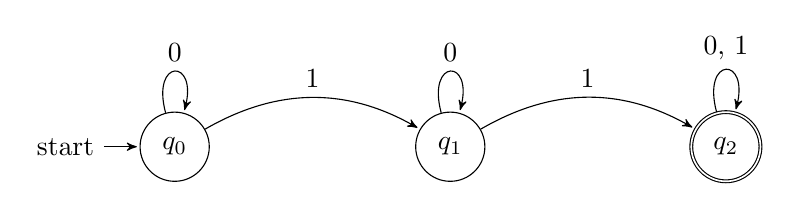
\begin{tikzpicture}[->,>=stealth',shorten >=1pt,auto,node distance=3.5cm]
  \node[initial, state]   (q0)                {$q_0$};
  \node[state]            (q1) [right of=q0]  {$q_1$};
  \node[state, accepting] (q2) [right of=q1]  {$q_2$};

  \path[->]
        (q0) edge [bend left]  node [above] {1} (q1)
             edge [loop above] node [above] {0} (q0)
        (q1) edge [loop above] node [above] {0} (q1)
             edge [bend left]  node [above] {1} (q2)
        (q2) edge [loop above] node [above] {0, 1} (q2);
\end{tikzpicture}
    \end{solution}}
\ifprintanswers
\else
    \newpage
\fi

  \part Welche Aussagen sind korrekt?
  \begin{checkboxes}
    \choice $0100 \in L(M)$
    \CorrectChoice $\hat{\delta}(q_0, 011011) \in F$
    \CorrectChoice $L(M) = \{w \in \Sigma^* \mid \hat{\delta}(q_0,w) \in F\}$
    \CorrectChoice $\hat{\delta}(q_0, 011011) = \hat{\delta}(q_1, 00001)$
    \choice $\hat{\delta}(q_0, 011011) = \hat{\delta}(q_0, 010000)$
  \end{checkboxes}

  \part
  Bestimme $L(M)$.
    \uplevel{\begin{solutionorbox}[5em]$ $\\
      $L(M) = \{w \in \{0,1\}^* \mid |w|_1 \geq 2\}$
    \end{solutionorbox}}

\end{parts}


\end{questions}
\end{document}
